\documentclass{beamer}
\usepackage[utf8]{inputenc}
\usepackage[T2A]{fontenc}
\usepackage[english, russian]{babel}
%\usepackage[sfdefault, light]{roboto}
\usepackage{epstopdf}
\usepackage[font={footnotesize}, labelfont={footnotesize}]{caption}
\usepackage[font={footnotesize}, labelfont={footnotesize}]{subcaption}
\usepackage{bm}
\usepackage[absolute,overlay]{textpos}
  \setlength{\TPHorizModule}{1mm}
  \setlength{\TPVertModule}{1mm}

\usepackage{tikz}

% Listings
\usepackage{listings}
\definecolor{codegreen}{rgb}{0,0.6,0}
\definecolor{codegray}{rgb}{0.5,0.5,0.5}
\definecolor{codepurple}{rgb}{0.58,0,0.82}
\definecolor{backcolour}{rgb}{0.95,0.95,0.92}
 
\lstdefinestyle{pythonstyle}{
    backgroundcolor=\color{backcolour},   
    commentstyle=\color{codegreen},
    keywordstyle=\color{magenta},
    numberstyle=\tiny\color{codegray},
    stringstyle=\color{codepurple},
    basicstyle=\scriptsize,
    breakatwhitespace=false,         
    breaklines=true,                 
    captionpos=b,                    
    keepspaces=true,                 
    numbers=left,                    
    numbersep=5pt,                  
    showspaces=false,                
    showstringspaces=false,
    showtabs=false,                  
    tabsize=2
}
\lstset{style=pythonstyle, language=Python}

\graphicspath{ {images/} }
\setbeamertemplate{caption}{\raggedright\insertcaption\par}
\def\figurename{}

\title{Scikit-learn: структура библиотеки и принципы проектирования}
\date[\today]{Практика по дисциплине <<Технологии ИИ>>\\\today}
\author[Anton]{Першин Антон Юрьевич, Ph.D. \\ Никольская Анастасия Николаевна}

\institute{Программа <<Большие данные и распределенная цифровая платформа>>\\Санкт-Петербургский государственный университет}

\usetheme{tonythequick}

\begin{document}

\begin{frame}
\titlepage
\end{frame}

\setcounter{framenumber}{0}

\section{}

\begin{frame}{Обзор Scikit-learn}
    \small

    Scikit-learn является easy-to-use библиотекой для машинного обучения, реализующей множество полезных методов.

    \begin{figure}[H]
        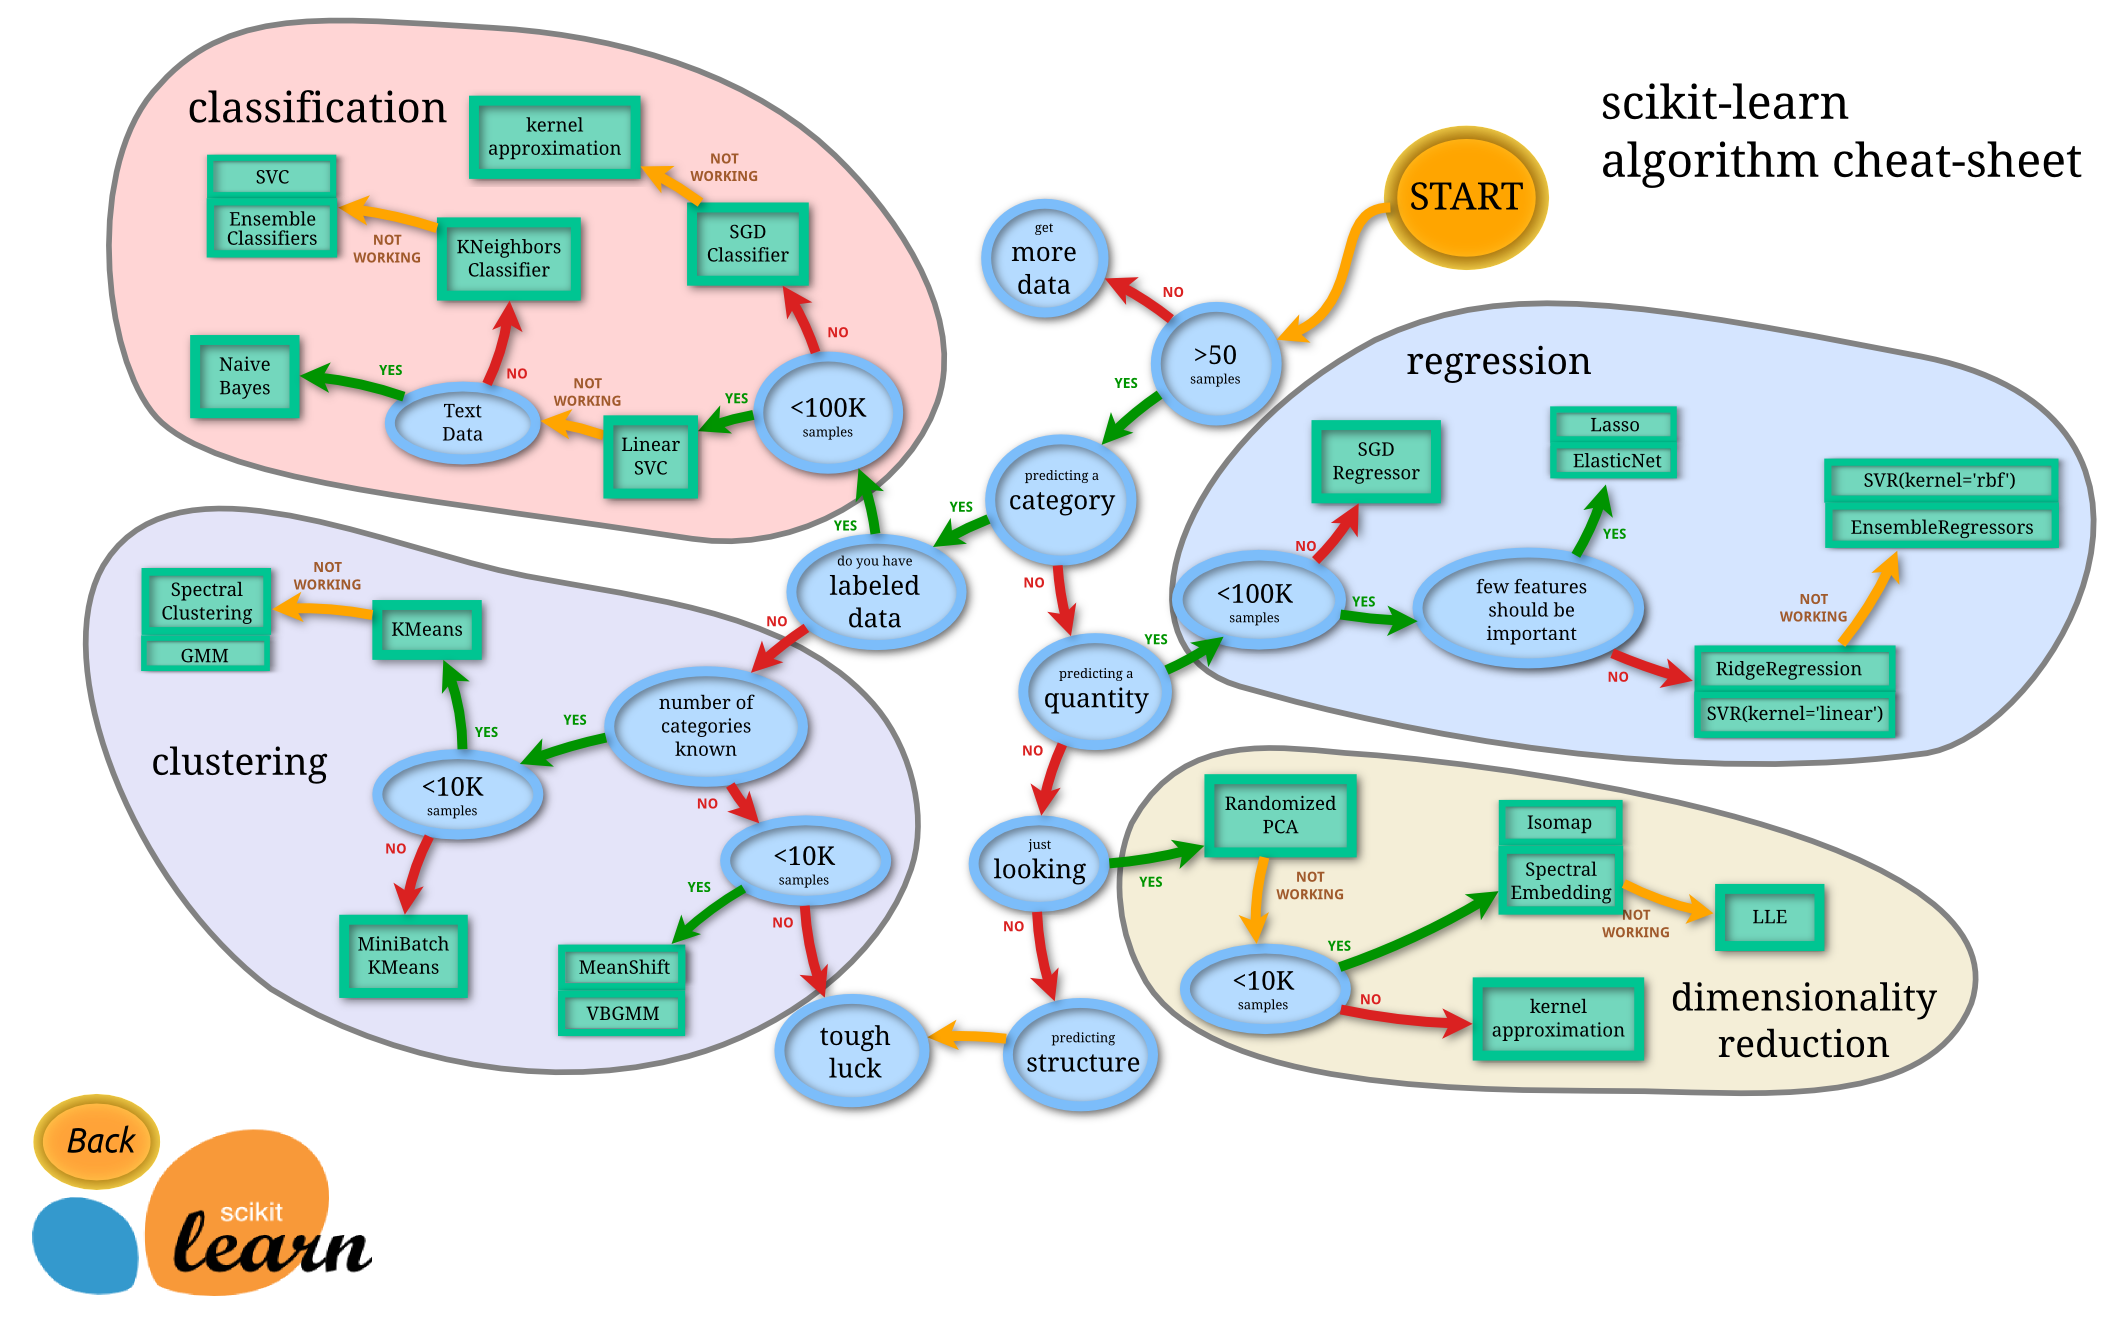
\includegraphics[width=1.0\textwidth]{sklearn_map.png}
    \end{figure}

\end{frame}

\begin{frame}{Обзор Scikit-learn}
    \small

    \texttt{Scikit-learn} обеспечивает следующую функциональность:
    \begin{itemize}
        \item Препроцессинг (обработка и преобразование признаков, их отбор)
        \item Понижение размерности (PCA, LLE, t-SNE etc.)
        \item Решение задач:
        \begin{itemize}
            \item регрессии (линейные модели, деревья решений, SVM, GP etc.)
            \item классификации (логистическая регрессия, деревья решений, SVM, etc.)
            \item кластеризации (k-means, MeanShift, BIRCH, DBSCAN etc.)
        \end{itemize}
        \item Создание мета-моделей (ансамбли: бэггинг, бустинг, стэкинг)
        \item Выбор моделей (кросс-валидация, поиск гиперпараметров)
    \end{itemize}
\end{frame}

\begin{frame}{Структура API Scikit-learn}
    \small

    Все объекты в \texttt{Scikit-learn} находятся в рамках общего API, который строится вокруг трех дополняющих друг друга интерфейсов:

    \begin{itemize}
        \scriptsize
        \item \textbf{Estimator} (строит и обучает модели)
        \item \textbf{Predictor} (выполняет предсказание/inference)
        \item \textbf{Transformer} (преобразует данные)
    \end{itemize}

    Общие принципы построения API \texttt{Scikit-learn}:
    \begin{itemize}
        \scriptsize
        \item \textbf{Consistency:} все объекты (простые и сложные) используют общий интерфейс, состоящий из ограниченного набора методов
        \item \textbf{Inspection:} все параметры, передаваемые на вход моделям и полученные во время обучения, сохраняются и доступны как открытые аттрибуты класса
        \item \textbf{Non-proliferation of classes:} специализированные классы используются только для моделей, остальные объекты представлены стандартными типами/классами (например, датасетами могут быть numpy массивы, разреженные scipy матрицы или датафреймы pandas)
        \item \textbf{Composition:} везде, где это возможно, модели реализованы так, чтобы их можно было использовать как ``строительные блоки'' других композиционных моделей
        \item \textbf{Sensible defaults:} все параметры моделей должны иметь ``разумные'' значения по умолчанию, чтобы модель можно было использовать для получения baseline решения
    \end{itemize}
\end{frame}

\begin{frame}[fragile]{Интерфейс Estimator}
    \footnotesize

    Любая модель \texttt{Model}, имеющая параметры, обучаемые на входных данных \texttt{X} и выходных \texttt{y}, должна реализовать интерфейс Estimator:
    \begin{enumerate}
        \item Отнаследоваться от \texttt{sklearn.base.BaseEstimator} (под параметрами здесь понимаются гиперпараметры, передаемые в конструктор)
        \begin{lstlisting}
class BaseEstimator:
    def get_params(deep=True):
        ...

    def set_params(**params):
        ...\end{lstlisting}    
        \item Реализовать \texttt{fit(X, y, **kwargs)}
    \end{enumerate}

    Пример использования:
    \begin{lstlisting}
X = np.random.randint(10, size=(1000, 2))
y = np.ones((1000, 1))
model = Model(hyperparameter=1e-3)
model.fit(X, y)\end{lstlisting}
        
\end{frame}

\begin{frame}[fragile]{Интерфейс Estimator}
    \footnotesize
    
    \textbf{Инициализация и обучение модели строго разделены:}
    \begin{itemize}
        \item \texttt{\_\_init\_\_()} принимает только гиперпараметры модели как явно заданные ключевые слова
        \item \texttt{fit(X, y)} принимает данные для обучения и возвращает \texttt{self}
    \end{itemize}

    \textbf{Параметры модели:}
    \begin{itemize}
        \item Гиперпараметры хранятся как аттрибуты класса
        \item Обучаемые параметры хранятся как аттрибуты с ``\_'' на конце
    \end{itemize}

    \textbf{Пример:}
    \begin{lstlisting}
class SubtractMeanAndShiftEstimator(BaseEstimator):
    def __init__(self, shift=0.):
        self.shift: float = shift
        self.means_: NDArray = None

    def fit(self, X: NDArray, y: Optional[NDArray]):
        self.means_ = X.mean(axis=0)
        return self\end{lstlisting}

    Практически все объекты в \texttt{scikit-learn}, преобразующие данные, являются Estimators
\end{frame}

\begin{frame}[fragile]{Интерфейс Predictor}
    \scriptsize

    Интерфейс Predictor расширяет интерфейс Estimator, добавляя к нему два метода:
    \begin{itemize}
        \item \texttt{predict(X\_test)} для предсказания по входным данным \texttt{X\_test}
        \item \texttt{score(X\_test, y\_test)} для оценки предсказания
    \end{itemize}

    \textbf{Пример:}
    \begin{lstlisting}
class SubtractMeanAndShiftEstimator(BaseEstimator):
    def __init__(self, shift=0.):
        self.shift: float = shift
        self.means_: NDArray = None

    def predict(self, X: NDArray) -> NDArray:
        e = np.ones((X.shape[0], 1))
        return X -  e @ self.means_.reshape(-1, 1).T + self.shift

    def score(self, X: NDArray, y: NDArray) -> float:
        return r2_score(y, self.predict(X))\end{lstlisting}
\end{frame}

\begin{frame}{Интерфейс Transformer}
    \small

    Интерфейс Transformer расширяет интерфейс Estimator:
    \begin{itemize}
        \item Обязательно: добавить метод \texttt{transform(X)} для преобразования данных \texttt{X}
        \item Опционально для работы с pipelines:
        \begin{itemize}
            \scriptsize
            \item добавить метод \texttt{get\_feature\_names\_out(input\_features=None)} для возвращения имен преобразованных признаков
            \item установить аттрибут \texttt{feature\_names\_in\_} во время вызова \texttt{fit()}
        \end{itemize}
    \end{itemize}

    Для создания Transformer полезными оказываются стандартные миксины:
    \begin{itemize}
        \item \texttt{sklearn.base.TransformerMixin}
        \item \texttt{sklearn.base.OneToOneFeatureMixin}
        \item \texttt{sklearn.base.ClassNamePrefixFeaturesOutMixin}
    \end{itemize}
\end{frame}

\begin{frame}[fragile]{FYI: миксины (mixins)}
    \small

    \textbf{Миксином} называют класс, расширяющий функциональность дочернего класса через ограниченную форму множественного наследования. Он не содержит собственных аттрибутов и не предназначен для создания экземпляров.
    
    \vspace{10pt}
    Рассмотрим пример базового Estimator:

    \begin{lstlisting}
class MyEstimator:
    def __init__(self, mean=0.):
        self.mean: float = mean

    def get_params(deep=True):
        return {"mean": self.mean}

    def set_params(mean=0.):
        self.mean = mean\end{lstlisting}
    
\end{frame}

\begin{frame}[fragile]{FYI: миксины (mixins)}
    \small

    Создадим миксин для вывода гиперпараметров:
    \begin{lstlisting}
class PrinterMixin:
    def __repr__(self):
        return "\n".join([f"{att_name}: {att_value}" for att_name, att_value in vars(self).items()])\end{lstlisting}

    Тогда Estimator с выводом гиперпараметров будет иметь следующий вид:
    \begin{lstlisting}
class PrintableEstimator(MyEstimator, PrinterMixin):
    def fit(X, y):
        return self\end{lstlisting}

    Порядок базовых классов в множественном наследовании важен: он влияет на MRO (method resolution order).
\end{frame}

\begin{frame}[fragile]{Композиция Estimators}
    \scriptsize

    \textbf{Последовательное объединение} Estimators: \texttt{sklearn.pipeline.Pipeline}

    \textbf{Параллельное объединение} Estimators: \texttt{sklearn.pipeline.FeatureUnion}

    \vspace{10pt}
    Все промежуточные шаги в Pipeline являются Transformers, а последний шаг -- любой Estimator

    \begin{lstlisting}
from sklearn.pipeline import Pipeline
from sklearn.preprocessing import StandardScaler
from sklearn.linear_model import LinearRegression


pipeline = Pipeline([
    ("scaler", StandardScaler()),
    ("regressor", LinearRegression()),
])
...
pipeline.fit(X, y)
y_pred = pipeline.predict(X_test)  # mimics the last estimator interface\end{lstlisting}

    Доступ к параметрам индивидуальных Estimators организуется с помощью синтаксиса \texttt{<estimator>\_\_<parameter>}
\end{frame}

\begin{frame}[fragile]{Композиция Estimators через Pipeline}
    \scriptsize

    \begin{figure}
        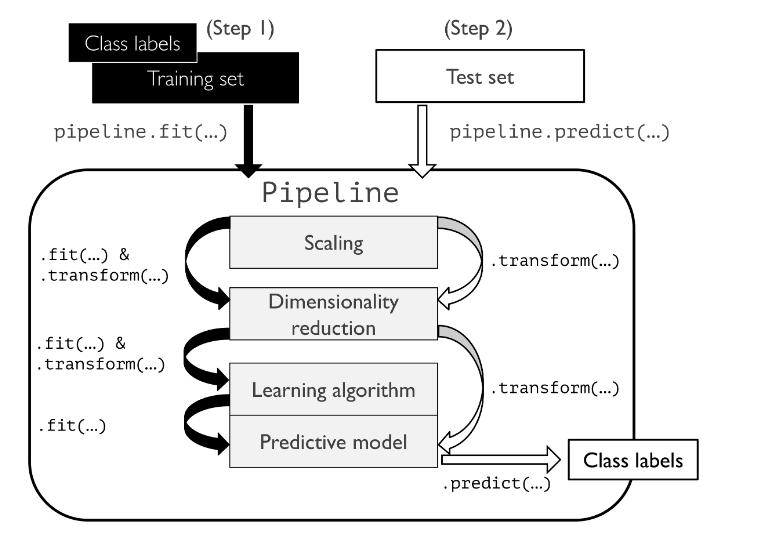
\includegraphics[width=1.0\textwidth]{sklearn_pipeline.png}
    \end{figure}
\end{frame}

\end{document}
